% Created 2020-10-13 Tue 23:21
% Intended LaTeX compiler: pdflatex
\documentclass[11pt]{article}
\usepackage[utf8]{inputenc}
\usepackage[T1]{fontenc}
\usepackage{graphicx}
\usepackage{grffile}
\usepackage{longtable}
\usepackage{wrapfig}
\usepackage{rotating}
\usepackage[normalem]{ulem}
\usepackage{amsmath}
\usepackage{textcomp}
\usepackage{amssymb}
\usepackage{capt-of}
\usepackage{hyperref}
\usepackage[russian]{babel}
\usepackage[T2A]{fontenc}
\usepackage[utf8]{inputenc}
\author{Макаров Сергей}
\date{\today}
\title{Оптимизация промежуточного представления для абстрактной интерпретации}
\hypersetup{
 pdfauthor={Макаров Сергей},
 pdftitle={Оптимизация промежуточного представления для абстрактной интерпретации},
 pdfkeywords={},
 pdfsubject={},
 pdfcreator={Emacs 27.1 (Org mode 9.3)}, 
 pdflang={Russian}}
\begin{document}

\maketitle

\section{Введение}
\label{sec:orgc8daa55}
\subsection{Мотивация}
\label{sec:org6eaf7f6}
\begin{itemize}
\item В современных решениях для анализа бинарного кода одни и те же задачи, в частности, декодирование команд и трансляция их в промежуточное представление, решаются каждый раз заново, для каждой частной задачи.
\item В рамках проекта Glassfrog предлагается унифицированный подход для решения задач декодирования процессорных команд, трансляции их в промежуточное представление и анализа полученного представления.
\item Для описания форматов файлов, формата и семантики машинных команд предлагается использование внутреннего языка спецификаций с расчётом на то, что поддерживать такие спецификации проще, чем код.
\item В качестве решения для задач анализа кода предлагается подход, основанный на теории абстрактной интерпретации.
\end{itemize}
\subsection{Glassfrog}
\label{sec:orgd93d2f9}
\begin{center}
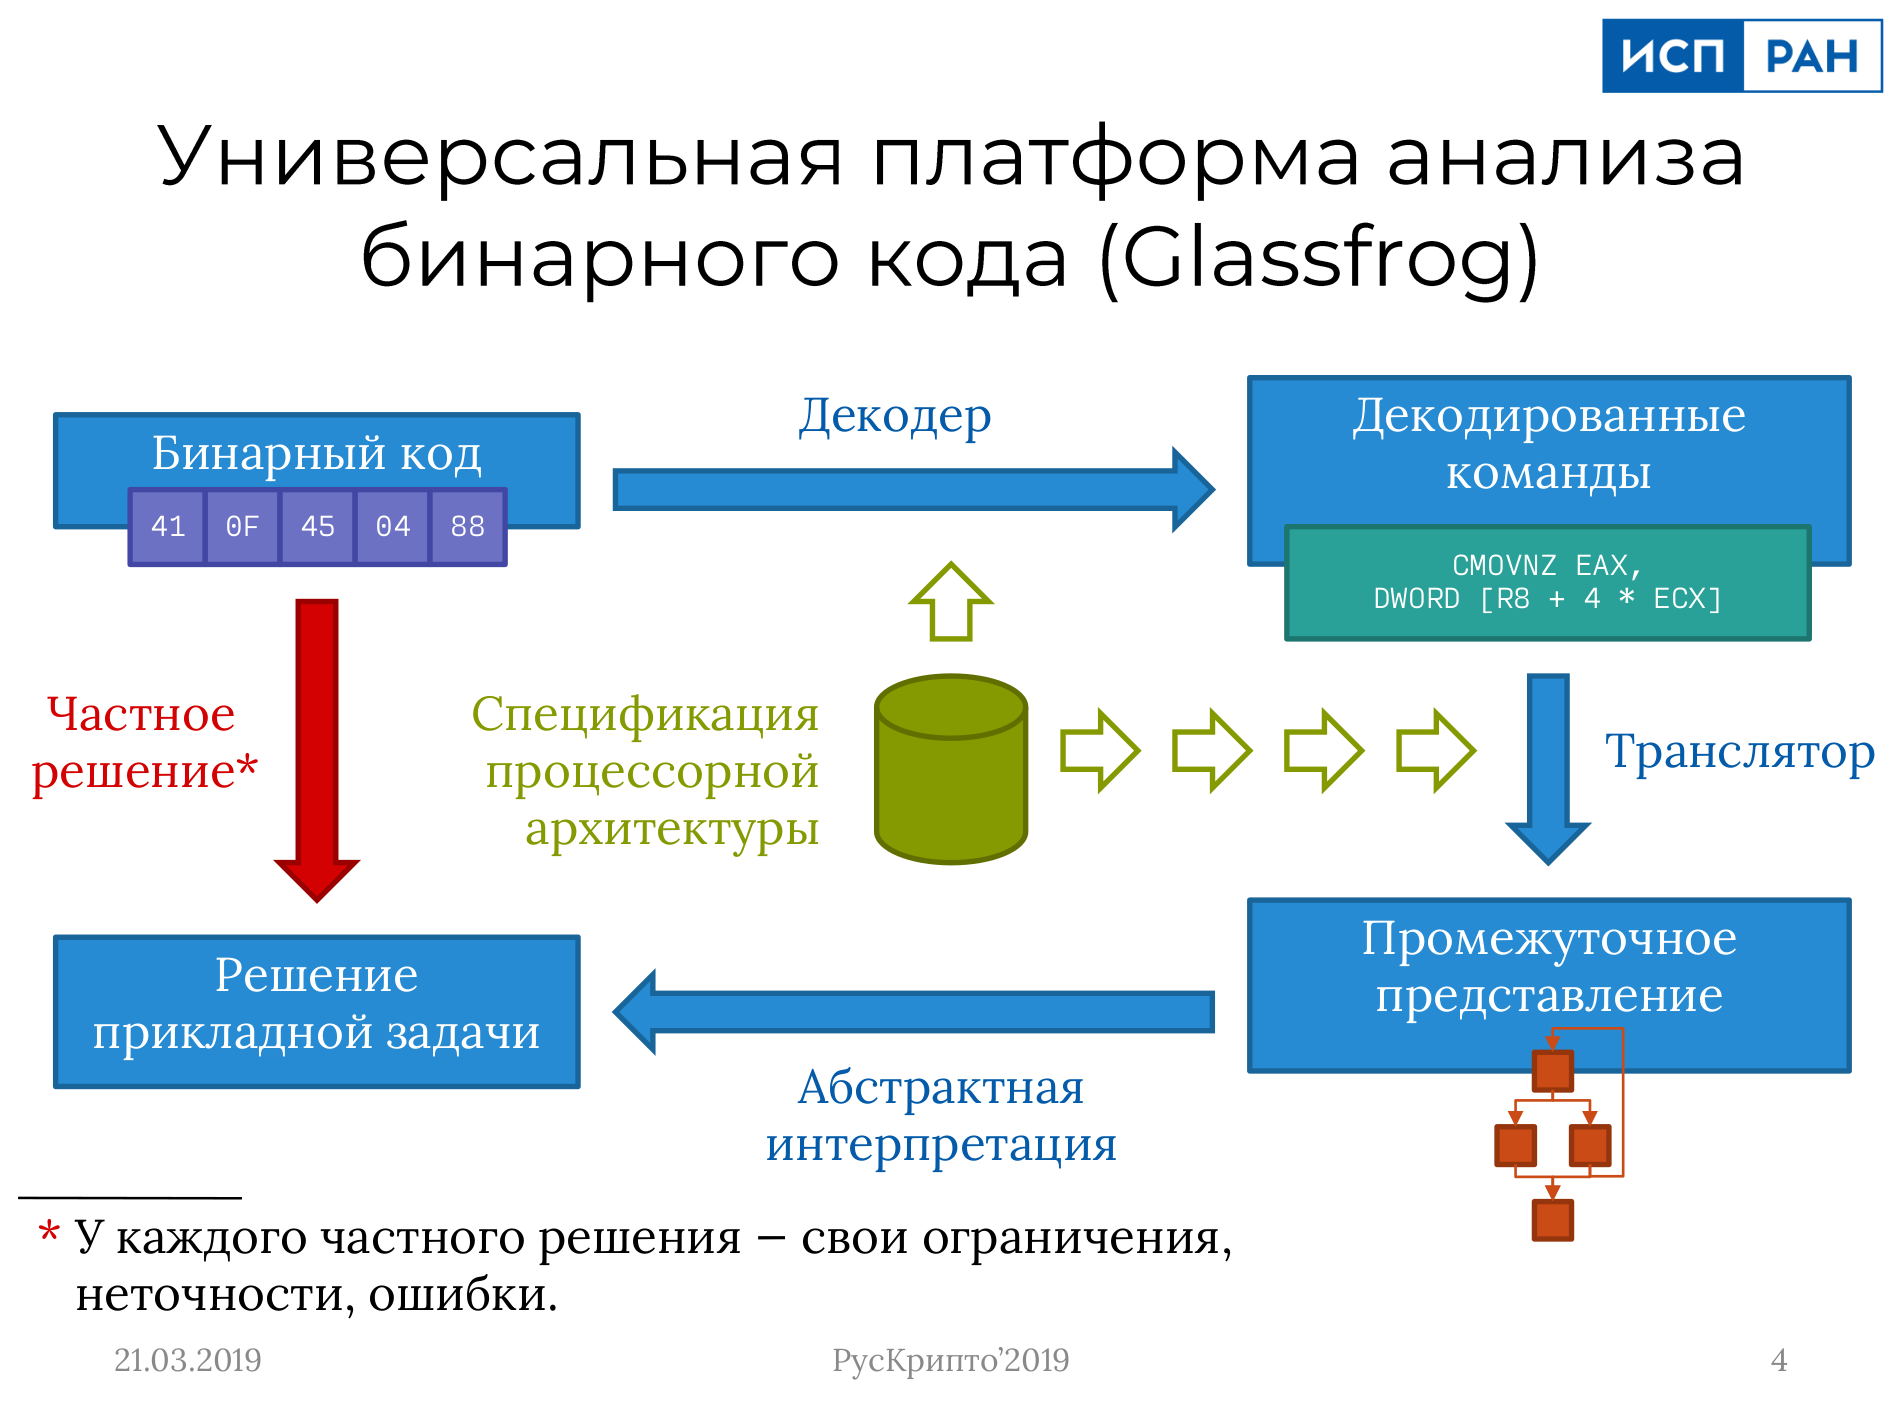
\includegraphics[width=.9\linewidth]{./glassfrog.png}
\end{center}
\subsection{Постановка задачи оптимизации}
\label{sec:orga68c8f8}
Поскольку сложность абстрактной интерпретации напрямую зависит от размера кода, имеет смысл перед абстрактной интерпретацией провести некоторые оптимизации, чтобы уменьшить размер промежуточного представления. Есть две возможности для оптимизации сгенерированного кода:
\begin{enumerate}
\item Оптимизация при компиляции спецификаций.
\item Оптимизация при построении промежуточного представления.
\end{enumerate}
\subsection{Структура Pivot2 IR}
\label{sec:orga4e2c98}
\begin{itemize}
\item Модули
\item Адресные пространства
\item Константы
\item Базовые блоки
\item Фрагменты
\end{itemize}
\subsection{Фрагменты}
\label{sec:org94f6bd8}
\begin{itemize}
\item Фрагмент представляет собой гамак из базовых блоков.
\item Фрагмент представляется в SSA форме. Передача переменных по рёбрам CFG осуществляется с помощью входных и выходных переменных базовых блоков.
\item Переменные базовых блоков имеют областью видимости весь фрагмент.
\item Базовые блоки представляют собой последовательность операторов. Всего есть 7 операторов: \texttt{APPLY}, \texttt{CALL}, \texttt{INIT}, \texttt{LOAD}, \texttt{MIX}, \texttt{SLICE} и \texttt{STORE}.
\end{itemize}
\section{Оптимизация спецификаций}
\label{sec:org77af76a}
\subsection{Общая структура оптимизаций}
\label{sec:orgb245074}
Трансляция спецификаций в IR происходит один раз, далее для анализа используются уже скомпилированные спецификации команд. Это позволяет провести основные трансформации на этом этапе.
\begin{enumerate}
\item Свёртка и продвижение констант проводятся на этапе семантического анализа.
\item Удаление лишних подвыражений и операторов \texttt{LOAD/STORE} производится на этапе приведения IR к SSA-форме.
\item Сворачивание цепочек операторов \texttt{SLICE} проводится отдельным проходом.
\item Наконец, финальным проходом проводится удаление мёртвого кода и упрощение графа потока управления.
\end{enumerate}
\subsection{Свёртка и продвижение констант}
\label{sec:orga71dee2}
Свёртка и продвижение констант производится на этапе семантического анализа. Для этого каждый узел AST, соответствующий выражению, снабжается атрибутом "значение". Эти атрибуты затем вычисляются отдельным проходом по AST. Если для узла AST значение уже вычислено, код для его вычисления не генерируется, и для соответствующей конструкции генерируется оператор \texttt{INIT}.
\subsection{Построение SSA}
\label{sec:orgf8a3024}
\begin{enumerate}
\item Обходятся все базовые блоки в CFG, переименовываются переменные в каждом операторе: входные переменные заменяются соответствующими им определениями, для выходных переменных формируются новые номера.
\item Устраняются лишние передачи переменных по рёбрам CFG, внесённые первой фазой.
\end{enumerate}
К полезным свойствам этого алгоритма относится то, что этот алгоритм позволяет применять локальные оптимизации во время построения SSA-формы. Более того, поскольку алгоритм не привязан к порядку обхода, это позволяет использовать оптимизации на расширенных базовых блоках. Кроме того, используя таблицу определений для переменных, можно также удалить все операторы \texttt{MIX}.
\subsection{Удаление лишних подвыражений}
\label{sec:org00b83f8}
Локальный Value Numbering:

Каждому оператору, вычисляющему некоторое значение (\texttt{APPLY}, \texttt{INIT}, \texttt{SLICE}), сопоставляется «выражение-значение». Поддерживается хэш-таблица, где ключами являются выражения-значения, а значениями -- переменные, в которых записаны результаты соответствующих операторов. При обнаружении оператора, соответствующее которому выражение-значение уже присутствует в таблице, оператор удаляется, а для его выходной переменной добавляется связывание с переменной, в которой это выражение было вычислено.
\subsection{Удаление лишних LOAD и STORE}
\label{sec:orgd45e06e}
Локальный Load/Store elimination:

Идея оптимизации состоит в том, что все чтения из памяти, в которую записано уже известное значение, можно исключить, используя это значение. Аналогично, можно удалить последующие записи значения в ту же память. Для этого поддерживается хэш-таблица, в которой ключами являются «выражения загрузки», содержащие адрес ячейки пространства, ссылку на адресное пространство, размер, и endianness доступа, а значениями являются переменные. Избыточные чтения и записи обнаруживаются и удаляются аналогично предыдущей оптимизации.
\subsection{Расширенные базовые блоки}
\label{sec:orgfc90214}
Расширенным базовым блоком называется максимальный по включению подграф графа потока управления с одним входным блоком и возможно несколькими выходными, такой, что у каждого его блока, за исключением может быть входного, не более одного предка.

Методы оптимизации, описанные в предыдущих слайдах, можно обобщить для расширенных базовых блоков. Для этого нужны две вещи: построить подходящий порядок обхода CFG, и исправить соответствующие методы.
\subsection{Обход расширенных базовых блоков}
\label{sec:org910cdfe}
Поддерживается массив «входных» блоков расширенных базовых блоков. На первом этапе он состоит только из входного блока. Затем на каждом этапе CFG обходится в глубину до блоков, у которых больше одного предка. Каждый такой блок добавляется в список «входных» блоков, если его ещё там нет. Как только обход EBB заканчивается, происходит переход к следующему, пока все EBB не будут пройдены.
\subsection{Обобщение методов оптимизации}
\label{sec:orgf62f093}
Заметим, что каждое выражение, описанное в блоке, доступно так же во всех блоках EBB, которые будут посещены при обходе EBB после захода в этот блок, но до выхода из него. 

Это позволяет предложить следующее обобщение для алгоритмов оптимизации:

Будем хранить таблицы «выражений-значений» и «выражений-загрузок» не в виде плоских таблиц, а в виде стека, каждый уровень которого представляет набор значений, которые доступны на данном «уровне» EBB. Расширенные базовые блоки обходятся в глубину, каждый EBB обходится по отдельности в глубину. При входе в базовый блок на стек загружается новый уровень, при выходе этот уровень сбрасывается со стека.
\subsection{Сворачивание цепочек операторов SLICE}
\label{sec:orge12e163}
Рассмотрим дерево, вершинами которого являются переменные, а ребро между переменными \texttt{u} и \texttt{v} существует тогда и только тогда, когда во фрагменте существует оператор \texttt{SLICE}, входом которого является переменная \texttt{u}, а выходом -- переменная \texttt{v}. В этом случае задача схлопывания цепочек операторов \texttt{SLICE} сводится к задаче «сжатия» ветвей в дереве.
\subsection{Сжатие ветвей}
\label{sec:orgdd3c82d}
\begin{enumerate}
\item Обход графа, нахождение всех цепей.
\item Разбиение подцепей на цепи, в которых промежуточные вершины не используются.
\item Сворачивание цепей в одно ребро.
\end{enumerate}
\subsection{Удаление мёртвого кода и упрощение CFG}
\label{sec:org14d83fb}
Удаление мёртвого кода производится с помощью классического Mark\&Sweep алгоритма. На первой фазе помечаются все важные операторы и переходы, на второй фазе непомеченные операторы удаляются.

Упрощение CFG достигается посредством систематического применения четырёх трансформаций:
\begin{enumerate}
\item Замена ветвления, оба ребра которого переходят в один блок, на безусловный переход.
\item Удаление пустого блока.
\item Слияние двух подряд идущих блоков.
\item Перенос ветвления из пустого блока к предку.
\end{enumerate}
\section{Оптимизация анализируемого кода}
\label{sec:org3cfaa5b}
\subsection{Абстрактная интерпретация}
\label{sec:org7363e64}
В терминах Glassfrog интерпретация это абстрактное состояние и набор передаточных функций, определяющих, как изменяется состояние при выполнении каждого оператора и при переходе по ребру CFG. Для задач анализа потока данных интерпретация должна быть монотонна, т. е. множество её состояний должно образовывать решётку. Вычисление результата абстрактной интерпретации по фрагменту происходит с помощью исполнителя.
\subsection{Глобальное удаление избыточного кода}
\label{sec:org0f9cef9}
С помощью абстрактной интерпретации находятся множества доступных выражений и содержимое памяти в начале каждого блока. Следующий проход заменяет лишние вычисления, чтения и записи на операторы \texttt{MIX}, используя эту информацию. Наконец, последним проходом удаляются операторы \texttt{MIX}.
\begin{enumerate}
\item Передаточная функция для операторов \texttt{APPLY}, \texttt{INIT} и \texttt{SLICE} добавляет соответствующее выражение как доступное.
\item Передаточная функция для оператора \texttt{STORE} обновляет содержимое соответствующей ячейки памяти.
\item Передаточная функция для оператора \texttt{CALL} сбрасывает наборы доступных выражений и содержимое памяти.
\end{enumerate}
\section{Заключение}
\label{sec:org7ebff81}
\subsection{Заключение}
\label{sec:org074f1e5}
\begin{itemize}
\item Были реализованы два пакета набора оптимизаций: для оптимизации спецификаций процессорных архитектур и для оптимизации анализируемого представления.
\item Замеров того, насколько реализованные оптимизации повышают скорость анализа, не производилось, поскольку соответствующая инфраструктура ещё не до конца реализована, и не набрана достаточная база примеров.
\item В дальнейшем планируется реализовать на основе инфраструктуры поиск утечек и пополнить базу примеров и спецификаций.
\end{itemize}
\subsection{Источники}
\label{sec:org7264934}
\begin{itemize}
\item \url{https://ispranproceedings.elpub.ru/jour/article/view/1120} \\
\item K. Cooper, L. Torczon, Engineering a Compiler 2nd Edition \\
\item \url{https://compilers.cs.uni-saarland.de/papers/bbhlmz13cc.pdf} \\
\item \url{http://www.di.ens.fr/\~cousot/COUSOTpapers/POPL77.shtml} \\
\item \url{https://ispranproceedings.elpub.ru/jour/article/view/1257}
\end{itemize}
\end{document}
